\documentclass[letterpaper,12pt]{article}
\usepackage{graphicx}

\begin{document}

This example demonstrates including graphics in a document. The SVG file will always need to be converted regardless of the engine used. The PNG file will need to be converted if the plain latex engine is used.

This document also demonstrates how makelatex handles bibliographies and has two different citations. Here are the first~\cite{chicago} and second~\cite{latexbook} citations.


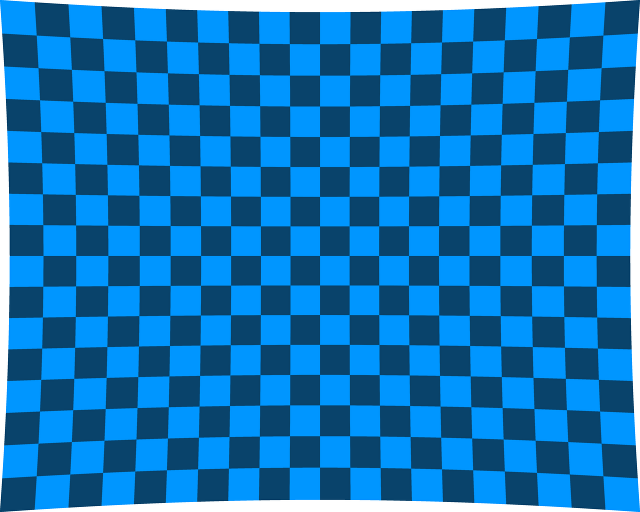
\includegraphics[width=.5\textwidth]{checkerboard}
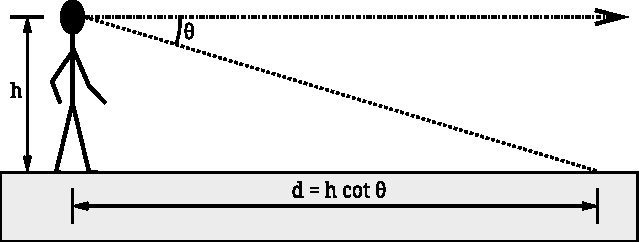
\includegraphics[width=\textwidth]{subdir/angle-of-decl}

\includegraphics[width=.1\textwidth]{red-circle}

\bibliographystyle{plain}
\bibliography{biblio}

\end{document}
